\chapter{Procedural Memory and the Lifecycle of Executable Skills}\label{ch:C15}

HyperSkill's 2026 implementation makes procedural memory an inspectable graph lifecycle: trajectory membership guides retrieval, skills and mistakes enter the execution view, and utility feeds later pruning and merging~\cite{xu2026hyperskill,repo_hyperskill2026}. The relevant scientific questions concern applicability, attribution, maintenance cost, and compatibility; neither a successful source trajectory nor a compact graph proves that its distilled procedure transfers.

\section{A procedure has preconditions and effects}\label{sec:C15:procedure}
A skill is reusable procedural knowledge that changes how an agent approaches a class of tasks. It can be a natural-language instruction, executable code, a workflow, or a package combining these forms. Its defining feature is a claim about applicability and action, rather than a claim about a fact alone. ``The repository uses a particular test framework'' is semantic knowledge; ``run this fixture before changing the parser'' is procedural guidance. A deployed skill can contain both, but the distinction matters when its environment changes.

Represent a candidate skill as $s=(P,\rho,Q,E,V)$, where $P$ is an applicability predicate, $\rho$ the procedure or policy fragment, $Q$ an intended postcondition, $E$ the evidence supporting it, and $V$ compatibility information. This is a proposed contract, not a requirement that every skill system exposes these fields. Natural-language skills often leave $P$ and $Q$ implicit. That makes them flexible but creates a risk that the policy applies a procedure beyond the conditions under which its evidence was collected.

Procedural memory is external to the model when it is stored and retrieved as an artifact. Activating the skill changes the model's conditional input; it does not necessarily change model parameters. A skill bank can improve performance with a frozen backbone, but that result should not be described as weight learning. Conversely, a procedure can later be distilled into parameters, changing its update, deletion, and verification boundaries. Chapter~\ref{ch:C30} treats the difference between these improvement targets.

The Agent Skills specification describes an artifact interface for instructions and resources~\cite{agentskills2026spec}. It is an interoperability and packaging reference, not empirical evidence that an agent chooses or executes skills correctly. A tool schema, a skill package, and a model parameter update are therefore distinct objects. A tool exposes an executable capability; a skill can tell the agent when or how to use capabilities; learning changes the policy that interprets both. Treating them as interchangeable makes attribution and authority ambiguous.

The institutional-knowledge perspective emphasizes that reusable procedures can encode local practices and constraints~\cite{corpus260314805}. Its case-study evidence should not be mistaken for a controlled estimate of productivity. The more general engineering implication is to attach scope and provenance to a skill rather than treating every successful local workaround as universally reusable knowledge. A workaround for one model's failure may become harmful after the model or tool interface is upgraded.


\section{Extracting procedures from experience}\label{sec:C15:extraction}
Repository-derived skills require a different evidential path from lessons extracted after an execution. A README describes an intended interface; a dependency manifest identifies a configured environment; an example demonstrates only the path it actually exercises. A proposed compiler should preserve those source roles, resolve referenced APIs at a pinned revision, and validate a minimal invocation in an isolated fixture before promoting the text into reusable guidance. Its output should state which preconditions were checked and which remain documentation claims. Successful package import does not establish that a remote operation is authorized or that an example's destructive defaults are appropriate. Repository instructions remain untrusted inputs during extraction. They cannot grant additional capabilities merely because the resulting package is called a skill. This separates source acquisition, executable validation, and activation authority.

An experience-to-skill pipeline takes a trajectory and constructs a reusable abstraction. The trajectory contains observations, attempted actions, failures, and an outcome; the abstraction identifies a pattern presumed to transfer. This is a causal inference problem under severe confounding. A successful episode does not identify which action caused success, and a failed episode does not prove that every included procedure was wrong. Outcome-conditioned extraction can help focus attention, but it cannot manufacture counterfactual evidence.

Let $Y$ be task success and $S$ indicate that a particular skill was made available. The difference $\mathbb E[Y\mid S=1]-\mathbb E[Y\mid S=0]$ is observational unless assignment is controlled or suitable identification assumptions hold. Familiar tasks can both retrieve a skill and be easier. A high success rate among retrieved uses can therefore overestimate causal value. The extraction system should retain the original situation and outcome rather than attaching an unconditional ``effective'' label to the resulting prose.

Positive strategies and negative lessons are also different memory objects. A negative lesson can specify a known failure pattern without prescribing a complete alternative. An agent should not convert ``this search query failed'' into ``never use this search tool.'' The abstraction must preserve the scope of the failure. Including environment version, task subtype, and the relevant precondition can prevent a local observation from becoming a global prohibition.

HyperSkill explicitly extracts subtask structure, reusable skills, and lessons from experience, organizing them through trajectory-level hyperedges~\cite{xu2026hyperskill}. Its retrieved memory is assembled for a task and then used during execution. This makes the mechanism different from a store that continually rewrites the prompt at every step. The task-level assembly boundary is important: a newly discovered fact or a changed tool contract during execution may require an additional update mechanism outside that fixed retrieved guidance.

A robust extraction implementation should separate parsing from admission. First construct a candidate object. Then validate required fields, source references, compatibility, and prohibited authority changes. Finally decide whether the candidate should be active, experimental, quarantined, or discarded. A malformed extraction should not silently fall back to a broad generic rule that is indistinguishable from a validated skill. If a fallback is used, record its origin so later evaluation can distinguish generated knowledge from successful parsing.

The proposed acceptance test for a procedure includes a positive task where it should apply, a near-neighbor task where its precondition fails, and a changed-environment task where the procedure must be revised or ignored. This tests selective transfer rather than simple memorization. A skill that improves the positive case while damaging the negative control has not established broad utility, even if average benchmark success rises.


\section{Hypergraphs preserve trajectory membership}\label{sec:C15:hypergraph}
HyperSkill represents subtask and skill nodes together with a hyperedge for each experience~\cite{xu2026hyperskill}. The hyperedge retains membership in a common trajectory and carries a task description, distilled lesson, and quality information. This is more specific than a claim that graphs improve memory. The representation keeps an association among several elements that were used together, whereas a flat vector store retrieves each element independently. The benefit must still be evaluated against matched retrieval and evidence budgets.

Let $V=V_u\cup V_s$ be subtask and skill nodes and let $E$ be trajectory hyperedges. A task query $q$ produces a decomposition $P(q)$. One retrieval route matches this decomposition to subtask nodes, then expands to incident hyperedges. A second route matches the task description to trajectory representations. Their union is
\begin{equation}
 E^*=E_{\mathrm{sub}}\cup E_{\mathrm{task}}.
\end{equation}
Candidate skills are members of those retrieved hyperedges. HyperSkill ranks them primarily through retrieved co-occurrence,
\begin{equation}
 \kappa(s)=|\{e\in E^*:s\in e\}|,
\end{equation}
with semantic similarity used for ties. These equations describe the inspected method, not a newly proposed retrieval result.

The representation should not be confused with a magical source of higher-order semantics. A hypergraph can be encoded as a bipartite incidence graph with explicit hyperedge nodes. What matters is retaining trajectory identity and membership, not the use of one graph library. A pairwise projection that discards hyperedge identity can lose which groups co-occurred together, while a representation that preserves the incidence relation can express the same membership. This is a structural deduction that sharpens the comparison axis.

The decomposition route can retrieve procedural analogies that differ lexically at the whole-task level. It can also amplify decomposition errors: if the generated plan misidentifies the task, it steers retrieval toward the wrong experiences. The task-level route provides a complementary signal but does not guarantee correction. A meaningful ablation holds total retrieved evidence fixed and compares task-only, subtask-only, and fused retrieval, with the same downstream model and prompt budget.

Co-occurrence is evidence of repeated use within retrieved experiences, not proof of causal usefulness. A generic skill can appear frequently because it was extracted from many tasks, while a rare exception-handling skill can be decisive. Frequency-based ranking and quality-based maintenance address different concerns. Their interaction should be inspected: pruning a rarely tested item, changing the set of retrieved edges, or merging broad skills can alter the candidate pool before the co-occurrence ranker runs.



Figure~\ref{fig:C15:overview} isolates the mechanism and its stated information boundaries.
\begin{figure}[!htbp]
\centering
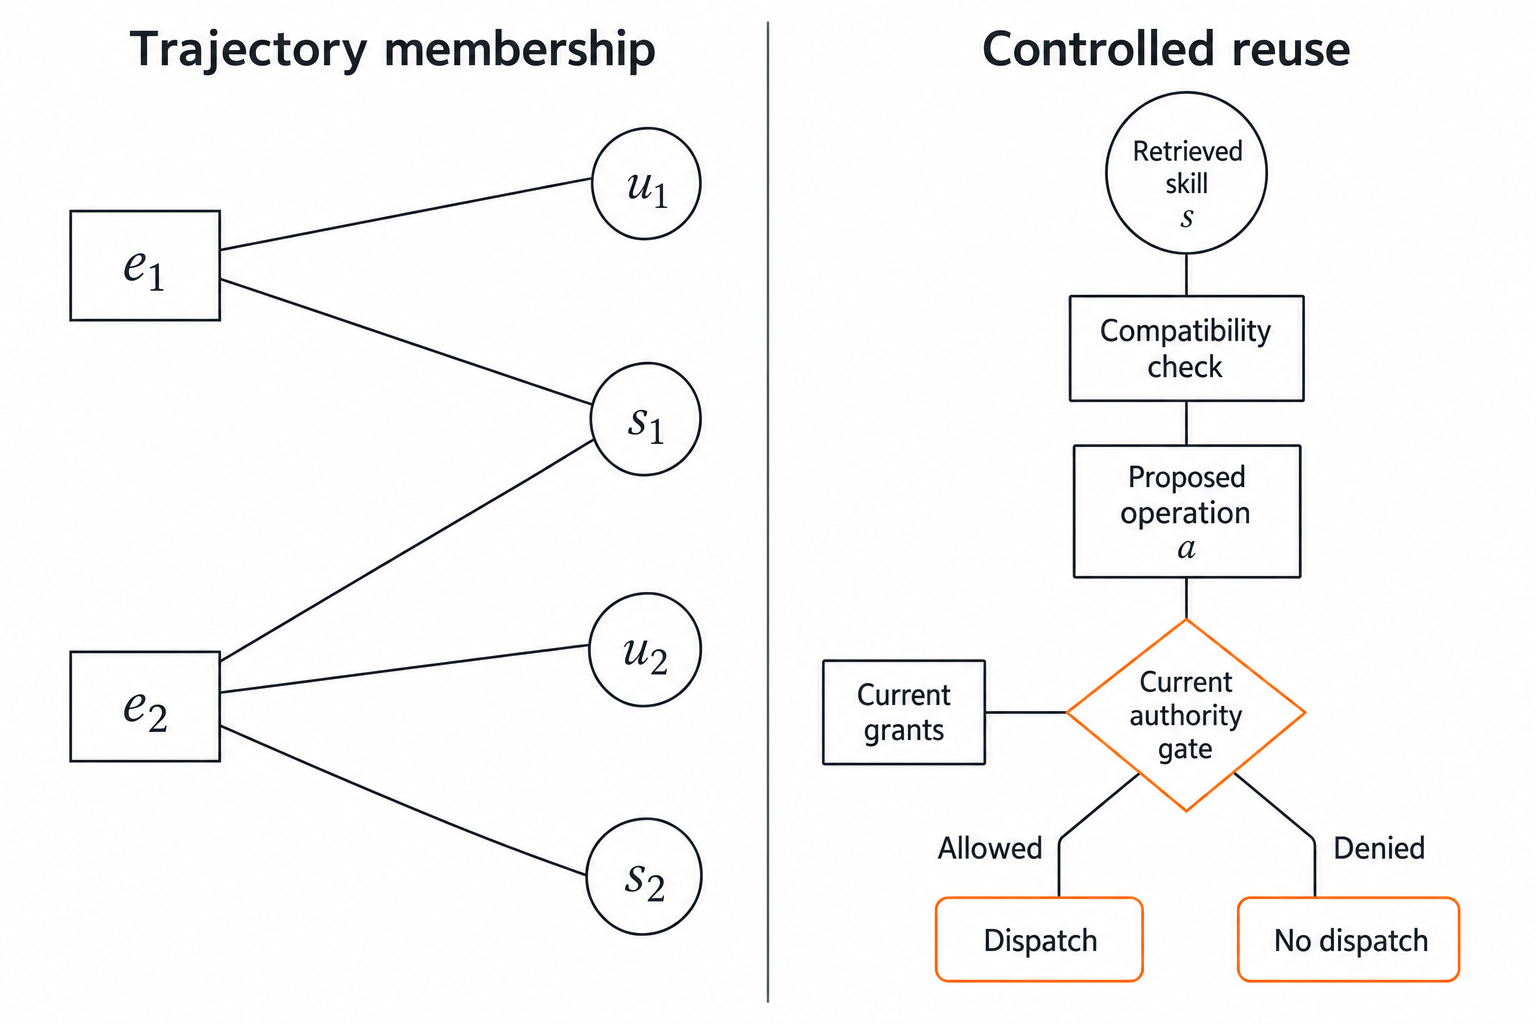
\includegraphics[width=\linewidth]{book/figures/assets/F15review.png}
\caption{An illustrative incidence representation: $e_i$ denote episodes, $u_i$ subtasks, and $s_i$ reusable skills. Undirected lines retain membership, not execution order. A retrieved skill remains a procedural hypothesis; compatibility and the proposed operation's current dispatch authority are separate checks. Neither membership nor compatible metadata proves procedural correctness. Maintenance uses additional evidence outside this schematic. Right-hand connectors show dependencies among checks and labelled conditional outcomes.}
\label{fig:C15:overview}
\end{figure}

\section{Quality-guided maintenance and its assumptions}\label{sec:C15:maintenance}
An accumulating skill bank can become redundant, stale, and internally inconsistent. HyperSkill periodically prunes low-utility knowledge and merges structurally related skills~\cite{xu2026hyperskill}. Its inspected code computes a utility score combining observed success rate with normalized step efficiency. For retrieval count $\nu$, success count $\sigma$, mean steps $\bar T$, and weight $\beta$, the form is
\begin{equation}
 \gamma=\beta\frac{\sigma}{\nu}
 +(1-\beta)\left(1-\frac{\bar T-T_{\min}}{T_{\max}-T_{\min}}\right),
\end{equation}
for $\nu>0$, $\beta\in[0,1]$, $0<\bar T$, and $T_{\min}\leq\bar T\leq T_{\max}$ with $T_{\max}>T_{\min}$, where the last two quantities delimit the step-count normalization range. The implementation handles untested nodes and degenerate ranges separately~\cite{repo_hyperskill2026}. This score is a maintenance heuristic. It is not an unbiased estimate of a skill's individual treatment effect.

The attribution problem is concrete. When several skills are retrieved together and a task succeeds, updating every retrieved node credits them jointly. A harmful item can survive because other guidance compensates for it. A useful item can be penalized on intrinsically difficult tasks. The quality estimate is policy- and task-distribution-dependent. If the model improves or the task order changes, old scores need not remain calibrated. Maintenance should therefore retain exposure counts and evaluation conditions rather than only a scalar utility.

The inspected \path{update_utility} updates retrieved nodes and their incident hyperedges after an episode. Its comment specifies that the utility is consumed by maintenance. The ranking routine still uses co-occurrence and similarity, not utility as its primary ordering~\cite{repo_hyperskill2026}. This separation is easy to miss in a high-level summary. Changing the utility formula affects which knowledge survives and merges; it does not simply replace the online ranker with a quality score.

The normalization has a time-dependent implementation boundary. The core maintains global historical extrema of observed mean step counts, but stores each node's utility when that node is updated; pruning later reads that stored value. Without a full rescore, nodes can therefore carry utilities computed under different ranges. This is a source-level observation, not a demonstrated benchmark error. A discriminating test holds one node's exposure and outcome counts fixed, changes the global range through an unrelated trajectory, and compares cached with recomputed utility before pruning. Versioning the scoring context or recomputing all eligible scores are possible interventions.

Structure-informed merging uses quality-weighted co-occurrence and propagated embeddings to propose related abstractions. A merged node can reduce redundancy, but it can also erase incompatible preconditions. The merge model should not decide compatibility solely from a high cosine score. Two procedures can use similar vocabulary while applying to different authorization scopes or tool versions. Retain source nodes or reversible merge metadata when the cost of a bad abstraction is high.

Maintenance frequency creates another tradeoff. Frequent updates can respond quickly to drift but add embedding, graph, and language-model work. Infrequent updates let redundant or harmful items influence more tasks. A maintenance schedule chosen on one benchmark order can overfit that order. Evaluate shuffled sequences, abrupt environment changes, and mixtures of easy and difficult tasks while charging all extraction and merge costs. Without these controls, a smaller final graph can look efficient even if its construction consumed substantial resources.

The practical lesson is to treat consolidation as a state transition with evidence and rollback. Pruned knowledge may still be relevant to historical audit, while merged knowledge should preserve references to the experiences that justified it. A physically compact bank is not necessarily a semantically safer bank.

Complexity depends on implementation rather than the hypergraph label. The inspected core constructs a dense quality-weighted co-occurrence matrix for the eligible abstraction nodes~\cite{repo_hyperskill2026}. For $n$ such nodes, matrix storage alone is $O(n^2)$ before propagated embeddings and merge candidates. If each of $m$ episodes contains at most $r$ eligible nodes, forming all within-episode pairs costs up to $O(mr^2)$ under a direct construction. These are analytic upper bounds for the stated representation, not timings. Sparse incidence operations can change the practical tradeoff, but a sparse source graph does not guarantee that the derived co-occurrence matrix stays sparse.

This matters when a memory method claims online scalability. Retrieval can remain fast while periodic maintenance becomes the dominant cost. The maintenance interval amortizes that work across tasks but also delays removal of stale knowledge. A benchmark ending just before maintenance can undercount the eventual cost; one ending just after it can overstate per-query latency if the work is actually asynchronous. Report cumulative maintenance time and resource use over the same task horizon, alongside the critical-path delay experienced by each task.


\section{An inspectable execution trace}\label{sec:C15:trace}
The inspected implementation supplies a concrete read-write-maintain path. \path{HyperSkillProvider.provide_memory} handles a memory request, obtains or generates a plan, invokes the hypergraph retrieval, and formats the resulting context. \path{take_in_memory} accepts a completed trajectory and performs outcome-conditioned extraction. In the core, \texttt{HyperGraph.retrieve} implements the task and subtask routes, while \path{maintain_graph} performs pruning, structural merging, orphan cleanup, and persistence~\cite{repo_hyperskill2026}. These are identifiable source functions at a pinned revision; they have been inspected, not executed here.

One feedback boundary deserves explicit validation. The provider reads the trajectory metadata field \path{is_correct} with a default of false. If a caller omits that field for an indeterminate outcome, the extraction path treats the episode as failure rather than as unknown~\cite{repo_hyperskill2026}. A wrapper claiming evidence-based consolidation should require a typed outcome $y\in\{0,1,\bot\}$, update outcome-dependent utility only for $y\ne\bot$, and retain unresolved trajectories separately. This is a proposed integration safeguard; it is not a claim that the paper's labeled evaluation omitted its outcomes.

Consider a constructed example with two past trajectories. One retrieved edge contains subtasks for locating a source, verifying its date, and comparing a claim, together with skills for checking primary evidence and preserving uncertainty. A second edge contains source-location and comparison subtasks plus a skill warning against treating a product announcement as a paper. A new research query matches both through its decomposition, even if the original task descriptions use different domain vocabulary. Co-occurrence ranks the shared evidence-checking skill above a skill appearing in only one edge, subject to the configured candidate pool.

This is an algorithmic illustration, not a benchmark observation. It makes two failure conditions explicit. First, if decomposition misses date verification, a relevant edge can fail to enter $E_{\mathrm{sub}}$. Second, if a generic skill appears in many retrieved edges, frequency can dominate a rare warning. The task route can recover some missed edges, but no guarantee follows from taking the union. Testing this example with controlled distractor edges would isolate a representation and ranking effect.

In the inspected core, the retrieval budget is divided between task-hyperedge candidates and subtask candidates. The subtask search overfetches candidates before filtering for the correct node type. Skills and mistakes are then ranked separately and limited separately. Consequently, the final guidance count and token count are not determined by a single nominal $k$~\cite{repo_hyperskill2026}. A cost comparison should inspect the actual formatted context rather than treating the retrieval parameter as the complete evidence budget.

The implementation also preserves instance-specific subtasks differently from abstract skills. Subtask insertion uses content-aware exact identity, while reusable abstractions can undergo semantic deduplication and structural merging. This distinction reflects the need to retain episode-specific planning context. It prevents one broad subtask label from automatically collapsing every occurrence, but it does not eliminate extraction or compatibility errors in the skill nodes.

A source-level reproduction should log the generated plan, retrieved subtask identifiers, task-route hyperedges, fused edge set, ranked skill and mistake identifiers, utility updates, and maintenance changes. These observables connect an outcome to the actual mechanism. Reporting only a final success rate and graph size would leave retrieval, extraction, and maintenance contributions difficult to distinguish.


\section{Reported results and unresolved attribution}\label{sec:C15:results}
HyperSkill evaluates multiple backbones on xBench, GAIA, and WebWalkerQA~\cite{xu2026hyperskill}. Table~\ref{tab:C15:hyperskill} records selected author-reported success rates. The improvements differ across backbones and tasks, and some comparisons tie another method. The paper's table should therefore not be paraphrased as strict dominance in every configuration. These values are not independently reproduced in this monograph.
\begin{table}[htbp]\centering\small
\caption{Selected HyperSkill success rates (\%), author-reported~\cite{xu2026hyperskill}.}\label{tab:C15:hyperskill}
\begin{tabular}{L{38mm}rrr}\toprule
Configuration & xBench & GAIA & WebWalkerQA\\\midrule
Qwen3-30B-A3B, no memory & 46.00 & 32.12 & 39.41\\
Qwen3-30B-A3B, HyperSkill & 52.00 & 36.97 & 50.59\\
GPT-4o, no memory & 54.00 & 32.73 & 46.47\\
GPT-4o, HyperSkill & 62.00 & 44.24 & 51.18\\\bottomrule
\end{tabular}
\end{table}

Task success and step efficiency need separate interpretation. A skill can reduce steps by encouraging premature termination. It can increase tool calls while improving evidence coverage. The paper reports these quantities separately, and a reproduction should preserve them rather than declaring every shorter trajectory better. Extraction, planning, embedding, and maintenance costs are additional lifecycle components. Lower execution-step counts do not establish lower end-to-end expense.

The main setting uses outcome feedback for memory updates, including gold outcome information in the relevant evaluation configuration. This is stronger feedback than many production agents receive. A method can learn useful procedural memory with such feedback while remaining limited when outcomes are ambiguous or delayed. If a model judge replaces gold labels, the judge's errors become part of the memory update loop and can persist into later tasks.

The fixed task-order seed is another qualification. An evolving bank learns from earlier tasks, so order changes both available experience and estimated utility. Repeating model decoding under one order does not measure order robustness. A shuffled-order evaluation and an explicitly held-out transfer set would help distinguish a favorable curriculum from stable procedural transfer. The result should report variation across orders and initial banks, not only the final average.

Component ablations can also be causally ambiguous. Removing a hypergraph component may simultaneously change candidate retrieval, context length, and abstraction content. A clean structure comparison preserves candidate text and token budget while varying only the membership information. A clean maintenance comparison preserves retrieval and evaluates before and after specific prune or merge operations. The paper provides useful mechanism evidence, while these further controls remain proposed experiments rather than additional reported results.

The evidence supports studying structured experiential memory as an implementable mechanism. It does not establish that higher-order storage universally outperforms flat retrieval, that the learned procedures remain valid after a model upgrade, or that recursive improvement accelerates indefinitely. Those stronger conclusions require new controls and different horizons.


\section{Compatibility authority and the skill supply chain}\label{sec:C15:compatibility}
A skill package can modify how an agent interprets tasks, chooses tools, and handles errors. It is therefore part of the effective policy surface. The package's text may be external data, but loading it into a privileged instruction position can give it operational influence. Compatibility and authority should be checked before activation, rather than inferred from a familiar name or a high retrieval score.

A proposed compatibility relation is $\mathrm{Compat}(s,\theta,h,\mathcal T,A)$, involving the skill, model, harness, tool set, and authorization. The relation can require specific tool schemas, artifact formats, and environmental preconditions. It can also forbid a skill from broadening authority. A procedure that was safe when a tool was read-only can become unsafe if the same name later exposes write effects. Version pinning makes this change detectable but does not prove semantic equivalence across versions.

The current Agent Skills format distinguishes required descriptive metadata from optional compatibility and tool declarations. In particular, its \path{allowed-tools} field is experimental and support varies by agent implementation; structural validation checks the artifact format, not every execution permission~\cite{agentskills2026spec}. A consumer must bind package content and referenced resources to the activated version and declare which fields it actually enforces. A description that says a tool is approved cannot override the dispatcher's current policy. Likewise, loading instructions on demand is a context-state transition under a fixed interpreter; changing executable skill resources changes the governing artifact version.

Progent provides a complementary enforcement principle: tool admissibility is checked by a symbolic policy, with policy expansion distinguished from narrowing~\cite{corpus250411703}. A retrieved skill should not silently expand that allowed action set. Even if the model interprets the skill as an instruction to use a new resource, the monitor can require an authorized scope change. This separates useful procedural guidance from the authority to produce effects.

Persistent procedural attacks exploit exactly this boundary. A malicious or mistaken lesson can survive many sessions and influence tasks whose original user never saw the source. Skill provenance should therefore include the generating trajectory, extractor, feedback source, validation results, and activation history. Repeated retrieval is not independent endorsement. A skill created by another agent is evidence from that agent, not a direct observation by the current one.

Consolidation can spread a defect. If a poisoned skill is merged into a broader procedure, simple deletion of the original node may not remove its influence. Record dependency links through merges and re-extractions. On revocation, invalidate affected descendants and test whether cached prompts or preloaded profiles still carry the procedure. The relevant guarantee is the actual scope of future-use prevention, not an unsupported claim of erasing every trace.

The proposed release gate for a skill includes schema checks, negative applicability cases, authority-preservation tests, representative task validation, and a rollback reference. These checks do not guarantee correctness for all future tasks. They make the acceptance conditions reviewable and reduce the chance that a single unverified episode becomes globally active procedural policy. Chapter~\ref{ch:C28} examines the broader attack and defense setting.


\section{Consolidation as controlled hypothesis revision}\label{sec:C15:synthesis}
The most useful interpretation of a skill bank is a collection of procedural hypotheses with evidence, rather than a set of permanently true rules. A new episode can support, narrow, contradict, or leave unchanged a procedure's applicability. Consolidation should preserve those possibilities. Automatically rewriting every new outcome into a confident lesson makes the bank vulnerable to noise, evaluator error, and shifting environments.

One proposed evaluation separates selection from revision. Freeze the initial bank and measure which skills are retrieved on held-out tasks. Then allow extraction while keeping retrieval fixed. Finally enable maintenance. This sequence identifies whether improvements arise from better access, new content, or pruning and merging. Charge the full cost at each stage and keep the same task order for the paired comparison, then repeat across randomized orders. This is a design for causal diagnosis, not a claim that every effect can be independently identified with a small experiment.

For a candidate merge, retain the original nodes as an experimental control. Evaluate the merged procedure on tasks where each original should apply and on tasks where their preconditions differ. If merging improves average performance but causes violations in the distinguishing cases, the abstraction has traded specificity for coverage. That tradeoff should be reported explicitly. A compact graph with fewer nodes can be easier to serve while preserving a less useful decision boundary.

Harness$^2$ illustrates a neighboring improvement target: task-level harness adaptation and reuse of experience about such adaptations~\cite{corpus261014224}. Its bounded task experiments differ from HyperSkill's explicit procedural-memory organization. Both can alter future behavior around a model without establishing an improvement in the model's own learning algorithm. The relevant comparison is what gets updated, which feedback selects it, how much extra execution is used, and whether held-out gains survive. Labels such as ``self-evolving'' do not settle those questions.

An original cross-layer deduction follows. The lifetime of a skill should be constrained by the lifetime of its assumptions. Tool version, environment behavior, model interpretation, and authorization can each invalidate a procedure without making its original episode false. This suggests expiring reusable status separately from deleting historical evidence. A later agent can still study why the skill once worked while being prevented from applying it automatically under changed conditions.

Trajectory multiplicity creates a distinct ranking sensitivity. Suppose a bank retains $k$ additional, separately identified copies of a retrieved trajectory containing skill $s$, and those copies survive candidate selection. The count rule above becomes $\kappa'(s)=\kappa(s)+k$ even though no independent experience was added. A competing skill absent from that trajectory receives no corresponding increment. This construction is conditional on retaining and retrieving the copies; it does not assert that the inspected implementation necessarily admits a particular duplicate. It identifies a test for exposure concentration: duplicate an episode's representation without changing its factual content and inspect ranking and downstream behavior. Grouping evidence by source lineage or normalizing trajectory contributions are possible interventions, whose effects on rare useful experience would also need measurement. Co-occurrence, independent support, and causal utility remain different quantities.

Conditional skill evidence can compose only under retained preconditions. Suppose a workflow has $K$ stages and $F_j$ is failure at stage $j$. If, for every reachable preceding success history under the evaluated configuration,
\begin{equation}
 P(F_j\mid F_1^c,\ldots,F_{j-1}^c)\leq\epsilon_j,
 \qquad 0\leq\epsilon_j\leq1,
\end{equation}
then the chain rule gives
\begin{equation}
 P\!\left(\bigcup_{j=1}^{K}F_j\right)
 \leq1-\prod_{j=1}^{K}(1-\epsilon_j)
 \leq\sum_{j=1}^{K}\epsilon_j.
\end{equation}
No independence assumption is required, but the conditional bounds must hold for the composed workflow, not merely for each skill on its original marginal task distribution. A tool migration, shared memory update, or changed predecessor can invalidate that premise. Finite test estimates need their own uncertainty bounds; a stored utility scalar is not such a certificate. Mandatory authorization remains a separate enforced precondition.

Procedural memory thus connects representation, retrieval, control, and governance. Its promise is selective reuse of experience; its central risk is selective reuse of an abstraction whose scope was never established. The rigorous engineering response is not to avoid skill banks, but to make their preconditions, evidence, revisions, costs, and failures part of the technical object being evaluated. Retrieval in Chapter~\ref{ch:C16} determines which of these hypotheses reaches the next decision.

